\chapter{Entrepreneurship and the entrepreneurial function} 
\label{ch:entrepreneurship}

If the division of labour is at the centre of the relational perspective, then its evolution is important in our discussion. Section~\ref{sec:socio-economicspace} noted that the development of a socio-economic space and the structure of the division of labour depends on two forces: one force that informs the division of labour and the other force that actively influences the division of labour. The first force regards the embeddedness of economic agents into some governance system that exists within the socio-economic space. The governance system---which consists of all embedded socio-economic institutions---informs the context of all economic interactions and relationships within the space, as well as socio-economic roles and production possibilities for individuals and firms. Therefore the division of labour, and thus the socio-economic roles attainable within society, is ultimately informed by the accepted governance system of the space. 

The second force regards entrepreneurship, which propigates a change to the socio-economic space by modifying elements of the prevailing governance system. Elements of the governance system can be influenced through entrepreneurial actions and the division of labour subsequently extended; an initial insight made by \citet{Smith1776}. Outlining a theory of the entrepreneur, and with it a theory of the entrepreneurial function within the relational perspective, is a main focus of this chapter.

After outlining a theory of the entrepreneur within the context of the relational perspective we illustrate the notions of entrepreneurship and the entrepreneurial function with an empirical example from history: the rise of the \emph{House of Medici}. Raymond de Roover's investigation into the rise and fall of the Medici Bank has become one of the most acclaimed pieces of business history. His analysis chronicled the evolution of the House of Medici from its establishment by Giovanni di'Bicci de'Medici, and later growth by his son Cosimo de'Medici. This case study approach, although deficient in overarching theory, provides an impressively intricate analysis of the financial accounts and business practices of the Medici Bank. The chapter therefore contributes to the work on the House of Medici by developing a theoretical overview of entrepreneurship and applying it to the actions of the entrepreneurial agents that drove the rise of the Medici Bank. Our specific application assesses the actions of Giovanni di'Bicci de'Medici and his son Cosimo di'Giovanni de'Medici. Although much has been written regarding the rise and fall of the Medici Bank there are none, to our knowledge, that specifically apply general theoretical models of entrepreneurship to this case study.

% Emiliya: p. 134 typo (paBrownloaw --> paper, Brownlow)

This chapter follows an analytical narrative approach inspired by `new business history'. The focus of new business history, according to \citet{JongHigginsDriel2015}, is to complement the case study research with a theoretical foundation. The focus on single firms within business history is not the source of the methodological problems faced by business historians. Studying single firms may highlight the need for more general models. In a recent paper, \citet{Brownlow2015} acknowledged the call of De Jong et al. for a new business history. In doing so Brownlow provides an analytic narrative regarding the establishment of the \emph{DeLorean Motor Company} in Northern Ireland circa 1975--1981, after the infamous `Troubles', a term associated with the ethno-nationalist conflict. Brownlow provides a convincing depiction of DeLorean as a rent-seeking entrepreneur who exploited Government policies and institutional responses to the deficient Northern Irish economy relative to the rest of Britain. The use of the analytic narrative illustrates the application of entrepreneurship is an important methodology, and one that we will use after outlining the entrepreneurial theory.

We take much inspiration from Brownlow and also note the call from De Jong et al. by investigating the Medici case with the proper methodology developed within the relational perspective. We provide an assessment regarding the entrepreneurial actions of the Medici Bank by investigating its establishment and prominence under the guise of institutional entrepreneurship. Specifically we provide a holistic perspective of entrepreneurship and the entrepreneurial function within a socio-economic space built from the basis of Schumpeter, Burt, Baumol, and Henrekson \& Sanandaji. By doing this we add some theoretical perspective to the business history contributions by de Roover and others regarding the rise of the Medici bank, the change in both the informal and formal perception of usury during this time, and the partnership system architecture of banking during this time. In undertaking this we cover institutional and entrepreneurial theories.

\subsubsection{Motivating an analytic narrative of the Medici}

The standard approach of economists in motivating an in-depth investigation is to formulate a set of puzzles. A number of interlinked puzzles can be identified when considering the establishment and rise of the Medici bank and the change in the institutional structure of Florence and Italy during this time. The first regards the institutional change regarding money-lending and the provision of financial credit that allowed it to move out of the ghettos in Florence to become the legitimate preserve of banks. This transition was symbolised by the rise of international money-lending and the rise of the Medici bank.

The second puzzle regards the phenomenal economic prosperity of the Medici bank and the political dominance of the Medici family across two generations of the family. The Medici family rose from obscurity to become one of the most powerful families in Europe. Prior to 1394---the establishment of the Medici bank---the Medici family were renowned criminals in Florence. Indeed, within a seventeen-year period five members of the Medici clan were sentenced to death by the criminal courts for capital crimes. The puzzles regarding the rise of the Medicean hegemony are addressed with respect to an analyses of entrepreneurship within the relational perspective; which regards economic actors who actively motivate a change to the governance system of the socio-economic space. In relation to this we look also to the interrelationship between the political and economic spheres of the economy, and how the Medici rose to dominate these spheres of the economy.

Beyond the economic puzzles noted, the motivation for analysing the Medici is related to the fact that there exists few other entrepreneurial families that have had such an impact on the cultural and economic composition of an Age than the Medici family. It is certainly debatable to suggest whether the world we see today would have been the same if the Medici had not come to such power in Florence during the late Middle Ages. It is of interest to see how a family gained so much economic and political control; how the actions and innovations of a small group punctuated the direction of a civilisation. More specifically, it is important to see how a model of the entrepreneur can explain how individuals attain power within a relational economy. The Medici were able to amass so much power and success due to their entrepreneurial ability: their potential to innovate, network, and create their own subjective socio-economic role within the Florentine socio-economic space enabled them to attain high levels of wealth and prestige.

\paragraph{Chapter outline.}

Section~\ref{sec:PerspectivesEntrepreneurship} provides an outline of the existing theory regarding entrepreneurship. Next, Section~\ref{sec:RPEntrepreneurship} integrates the notion of entrepreneurship to that of institutions and the governance system. From this we combine our perception of the relational perspective with the entrepreneur to discuss a more holistic perspective of the entrepreneur and entrepreneurship within the relational perspective. Section~\ref{sec:HouseofMedici} applies the notions developed to the case study of the rise of the Medici bank. Finally, Section~\ref{sec:ConcludingPoints} concludes.

\section{Theoretical perspectives of entrepreneurship}
\label{sec:PerspectivesEntrepreneurship}

A classic perspective of the entrepreneur comes from the work of Frank \citet{Knight1921}. Knight's perspective claims that all forms of entrepreneurship must have `uncertainty' and `profit' involved. His central thesis suggests that entrepreneurs profit from the burdening of uncertainty. This notion of uncertainty corresponds to the definition it has been given throughout the thesis: uncertainty relates to one-off events whose probability and outcome can only be subjectively estimated. Unlike risk, uncertainty cannot be estimated and insured against. Profit is the reward for those willing to bear unmeasurable, inestimable and uninsurable uncertainty rather than measurable, estimable and insurable risk. Entrepreneurs are thus those who are willing to incur the uncertainty of a potentially profitable course of action. This distinction between risk and uncertainty typically does not, however, filter into traditional economic theory. As a consequence \citet[p.~282]{Knight1935} notes that, ``in the idealised society of equilibrium theory, there would be no occasion for assigning the distinctive name of profit to any type of return.''

Traditional economic theory has suffered in the past from a failure to state clearly the role and actions of the entrepreneur. The persistent words of William \citet[p.~66]{Baumol1968} summarise how traditional economics has investigated this elusive economic entity since the Marginalist Revolution: ``The theoretical firm is entrepreneurless--the Prince of Denmark has been expunged from the discussion of Hamlet''. The consequence of this discrepancy should be underlined considering that some economists believe the entrepreneur to be the driving force of the prevailing capitalist ideology and economic prosperity \citep{Schmitz1989, WennekersThurik1999, Baumol2007}. Further, \citet[p.~1]{Lazear2002} suggests that, ``the entrepreneur is the single most important player in the modern economy.'' This omission within mainstream economics is certainly perplexing given its apparent importance. 

This section investigates three established theoretical perspectives of the entrepreneur and entrepreneurship. The first is that of occupational choice models and models of endogenous growth developed within the neo-classical framework. The second is the Schumpeterian perspective of capitalist economic development through the waves of creative destruction spurred by the entrepreneur. The final perspective is the Burtian perspective of the entrepreneur, developed on the basis that all economic activity is embedded in a social network.

\subsection{Traditional economics and occupational choice}

Ultimately, Baumol's argument is that the traditional theory of the firm does not allow for the integration of the entrepreneur. The production function suggests that the firm considers the costs and benefits attached to the employment of certain and well-defined factors of production including capital and labour. All firms within the industry optimise and operate at their profit-maximising equilibrium and subsequently provide an inert market structure producing output that already has a market attached. In the extreme case of perfect competition, certainty, homogeneity, non-existent barriers to entry, and individuality are assumed. A paradox follows whereby at the equilibrium of perfect competition there is no competition: all firms operate independently earning normal profit without being given the opportunity to innovate or undercut rivals. Innovation, reorganisation of trade networks, the leveraging of unique social networks, and product or process diversification are cast out of the equilibrium model. The eventual failure of marginal firms only derives from an exogenous change in the market as opposed to factors of uncertainty, bad networking, or poor managerial decision-making due to bounded rationality.

To suggest that neo-classical economics has continued to disregard the entrepreneur since the words of Baumol would be incorrect. Jean Baptiste Say initially coined the term around the beginning of the 19th Century \citep{Hindle2008}, claiming that the entrepreneur was an economic agent who owned a large quantity of resources and allocated them out of an area of lower into an area of higher productivity and greater yield. To a large extent, this perspective has been embraced by the neo-classical models. Indeed, the models of static equilibria provided mechanisms in which to integrate the individuals' decision to be an entrepreneur as an `occupational choice', meaning that individuals allocated their entrepreneurial talents to either becoming an entrepreneur and set up their own (homogeneous) firm or becoming an employee for an existing firm depending on the prevailing market wage level to the corresponding actions. The models from \citet{Lucas1978} and \citet{KihlstromLaffont1979} form the foundations of entrepreneurship as an occupational choice for economic agents.

Some deficiencies of occupational choice models are due to their market-centric foundation and assumptions. Specifically, equilibrium theories of the entrepreneur make three main assumptions. The first being that every economic agent can recognise all entrepreneurial opportunities, which derives from their \emph{ex ante} homogeneity. The second is that fundamental attributes about people--rather than information about opportunities or the encompassing structure of the socio-economic environment--determines who becomes an entrepreneur. Although human action is the result of individual ability there is no doubt that external and social factors also play a role on determining entrepreneurial action \citep{ShaneLockeCollins2003, AldrichMartinez2007}. Finally, they have the perception that being an entrepreneur is an occupational choice: that individuals can just choose to be an entrepreneur or not. The relational perspective developed above notes that most individuals cannot just `choose' to specialise in the role of an entrepreneur. Rather, it will be seen that individuals create their own role--they subjectively specialise--to their socio-economic environment. Indeed, they do not adopt a pre-existing occupation, but rather create their own and thus spur the deepening of the division of labour.

Endogenous neo-classical growth models have been created which include the notion of the entrepreneur \citep{Peretto1998, Sanders2007}. The most influential of which is the \citet{AghionHowitt1992} model and its later adaptations \citep{Aghion1997, HowittAghion1998} which facilitates the integration of entrepreneurial innovation as a driver of economic growth. Indeed, they do this by having firms invest resources in research to achieve a new product that renders the previous product obsolete. Capital is excluded from the basic model while economic growth results from technological progress, being a result of competition among firms that generate innovations. Firms are motivated by the prospect of temporary monopoly rents after a successful innovation is patented. Another innovation will again destroy these rents, as the `entrepreneur' is making the existing good obsolete. Although these are highly influential models created by Aghion and Howitt, and capture the Schumpeterian notion of creative destruction, they fail to capture the characteristics of the agent that leads to the destabilisation of the economy through the process of creative destruction--the entrepreneur. Indeed, although the 1992 article, for example, regards creative destruction as a driver of growth they do not mention the word ``entrepreneur'' throughout the article. Instead they simply suggest that it is the firm, investing in research and development, which drives technological advancement and therefore economic prosperity. This is undeniably true; firms that invest in research and development can create innovative products, but innovation still emerges from sources external of the firm. Again and again, it is seen that the neo-classical models' attempts to capture the entrepreneurial functions are continually ill-equipped.

The development of entrepreneurial models specifically built with the intention of encompassing institutional and social aspects are of paramount importance as the ultimate role. The perspective we develop of the relational entrepreneur will depend on the structure of the socio-economic environment. To this point we have seen that mainstream theory finds it difficult to model economic evolution through the entrepreneurial function. Below we will point to potential reasons why the mainstream theory finds it difficult to appropriately model economic evolution through the actions of the entrepreneur. I suggest that the problems of the traditional theory derive from the very axioms that underpin it: methodological individualism, methodological instrumentalism, and methodological equilibration. First we must extend our discussion of how economic theory perceives the entrepreneur by discussing the Schumpeterian and Burtian perspectives. From this basis we integrate institutional factors into entrepreneurship and provide a discussion of entrepreneurship within the relational perspective.

\subsection{Schumpeterian theory of the entrepreneur}

Although being progressively side-lined over previous decades \citep{Aldrich2005}, one of the most prominent perspectives of the entrepreneur comes from Joseph Schumpeter who discusses the entrepreneur and the entrepreneurial function in two places: the first is in chapter two of his book on economic development \citep{Schumpeter1934}; and the second is in a chapter prepared in 1928 for an economics handbook \citep{Schumpeter2003}. Schumpeter provides a novel perspective of the entrepreneur that is fundamentally differentiated from the neo-classical postulations. Realising the limitations of general equilibrium analysis in explaining economic evolution and development, Schumpeter rejects any notion of equilibria, instead emphasising that the economy needs to be analysed in a purely dynamic manner propelled by the waves of `Creative Destruction' \citep{Schumpeter1942}. From this basis he built a relatively loose conceptual model on the premise that even if markets were to approach equilibrium they would destroy it over time due to the advancement of product and process innovation. Through the entrepreneurial function new products and markets would be created thus provoking a deviation from the equilibrium point and the circular flow of the economy. The process of creative destruction as discussed by Schumpeter assumes that all entrepreneurial activity progresses the capitalist economic system; that the entrepreneur is a heroic entity productively influencing production and process techniques and providing new technologies and specialisations to the socio-economic space.

\subsubsection{Entwicklung and the entrepreneur}

Schumpeter's overall perspective of the entrepreneur fundamentally deviates from neo-classical economics, and thus Say's contribution of an individual that allocates resources in a more efficient manner. Instead, he initially took a more literal definition of the term entrepreneur as an individual who stimulated economic progress by finding new and better ways of doing things. In doing so Schumpeter emphasises the importance of innovation--a dynamic process that emerges from a stagnated state of affairs so that a new state of affairs can emerge--a concept notably absent from the neo-classical models of comparative statics, where the types of goods and services are given. Even the goods and services in the future are fully specified, which allows for inter-temporal trade. Production technology is also given. However, in emphasising innovation he took a relatively social perspective of the entrepreneurs' socio-economic environment. Moreover, he fully accepted that not every agent could be an entrepreneur. Each entrepreneurial agent specifically required two resources. The first resource was the existence of technical knowledge in order to produce new, innovative, outputs. Second, they required the power of disposal over the factors of production in the form of credit. In effect an entrepreneur requires specific forms of human capital for the development of relevant innovations, and also the sources of credit to fund its development and diffusion with the use of markets.

Considering this innovative and mutative quality, Schumpeter's acceptance of evolution--or \emph{entwicklung} \citep{Schumpeter2005}--is particularly notable. However, despite flirting with the concept of selection, Schumpeter did not follow his insights up with any major evolutionary discussion \citep{SmelsterSwedberg2005}. Further still, despite his efforts, he failed to provide any formal model in which to specifically link the entrepreneur, the entrepreneurial function, creative destruction, and economic development \citep{Witt2002}. He did however attempt to conceptually couple his discussion of the entrepreneur with one of internal economic development. He specifically saw that development was a process that emerged from actions endogenously occurring within the economy itself and not from the impact of some form of exogenous shock. An economy that was simply adapting to shocks that were exogenously endowed or were external to it was perceived as simply being dragged along by the changes in the surrounding world. This adaptation to an external or exogenous factor is not development. According to Schumpeter, economic development comes from innovative entrepreneurial action within the economy itself.

\begin{quote}
By `development' we shall understand only such changes in economic life as are not forced upon it from without, but arise by its own initiative from within... By this we should mean that economic development is not a phenomenon to be explained economically, but that the economy, in itself without development, is dragged along by the changes in the surrounding world, that the causes and hence the explanation of development must be sought outside the group of facts which are described by economic theory.
\begin{flushright}
Joseph \citet[p.~63]{Schumpeter1934}
\end{flushright}
\end{quote}

Despite his efforts to integrate the entrepreneur to endogenous economic development, Schumpeter largely failed to do so. As \citet{Becker2006} point out in the introduction of Development \citet[p.~111]{Schumpeter2005}, ``Development's dismissal of entrepreneurship as the explanation of discontinuities is the rare instance where Schumpeter himself indicates that he is still searching for an entirely adequate explanation of the novel social phenomena he had characterized as discontinuities.''

In discussing economic development, Schumpeter was adamant that development was not a self-organising process. Specifically he suggested that, ``[t]he economy does not grow into higher forms by itself'' \citep[p.~75]{Schumpeter2003}. When considering situations of increased complexity the difficulty of self-organisation becomes notable. Subsequently it becomes apparent that the entrepreneur does not just act as a diffuser of an innovation, but acts as an organising force that drives development of an economy from inside \citep{Marz1991}. Entrepreneurs actively organise society and the divisions of labour in the production of innovative outputs. With this, Schumpeter makes an interesting argument that homogeneous and fully autonomous agents may not necessarily produce systems that organise successful development when considering complex economies. Forces in terms of the entrepreneur and the government must actively organise society in fruitful production. Even if this organisation is imperfect or lacking fruitful development can still emerge.

\subsubsection{Personalisation and depersonalisation of the entrepreneur}

There remains an amount of controversy as to whether his perspective of the entrepreneur changed over time. There does seem to be an implicit distinction between what Schumpeter considered to be the entrepreneur, and what he considered to be the entrepreneurial function. However, his views on these are not mutually exclusive, he simply views the same innovative process from two different perspectives. In his latter work, Schumpeters analysis was extremely depersonalised, focussing on the process and outcome of the entrepreneurial function within the economy. In doing so, Schumepter placed more of an emphasis on the entrepreneurial activities and actions as opposed to the entrepreneurs' personal characteristics. \citet{BeckerKnudsen2003} implied that this made entrepreneurship seem to be a much more contingent activity; that the entrepreneurial function did not have to specifically emerge from a single individual, but may emerge from a group activity or a firm.

With respect to the depersonalised entrepreneurial function, Schumpeter stressed that the function of the entrepreneur is to reform or revolutionise the pattern of production. They can do this in many ways: by exploiting an invention or, more generally, an untried technological possibility for producing a new commodity or producing an old one in a new way, by opening up a new source of supply of materials or a new outlet for products, by reorganising an industry and so on. From this definition it is seen that the Schumpeterian entrepreneur is extremely firm-centric; providing the linkage specifically between the innovative function and firm organisation and output. Despite the difference in approaches, Schumpeter - like the neo-classical paradigm - stresses a direct link between the development of technology and resulting economic prosperity. However he suggested that technological advancement came from the fruition of an entrepreneur's innovative idea embodied within the economy and the production of heterogeneous output as opposed to a mere exogenous shock. This provides a general consensus that the entrepreneur is considered as an entity which blurred the distinction between macro and macro spheres of the economy: the entrepreneurial function was a microeconomic action with potential macroeconomic implications.

Under this definition Schumpeter contended that the entrepreneurial function, and thus the acts required to become an entrepreneur, was not the same as choosing an occupation or a profession. It is specifically not an occupational choice; one cannot learn to become an entrepreneur as if it were any other profession. To be an entrepreneur an agent must specifically carry out an innovative process, which is outside the predefined actions of a socially expected role. Thus being an entrepreneur is specifically converse to simply following the established institutions and subsequently conforming to a specific socio-economic profession. Moreover, Schumpeter contested that one should not be considered to be an entrepreneur forever; an entrepreneur should only be considered to be so during the period in which the agent is carrying out the innovative entrepreneurial function.

Schumpeter's earlier work looked more at the characteristics of the entrepreneur, or the `man of action', as an entity. In this text he considered the entrepreneur to be an exceptional, disruptive individual who actively \emph{disequilibriates} the economy with the introduction of new products or processes, thus carrying out the aforementioned entrepreneurial function. It is emphasised that entrepreneurial success is derived from the utilisation of an exogenous skill-set. In his first rendition of the entrepreneur he attributes almost superhuman powers of leadership to the entrepreneur. In many ways, he perceives the entrepreneur as an agent with innate talent; indeed, what differentiates a successful entrepreneur from other agents within the economy is their ability to lead a firm or act on an innovation. Much like the Lucas model, the entrepreneur is psychologically endowed with a form of `talent' or `leadership' that is exploited for successful entrepreneurship. In all, the exogenously endowed characteristic attributes of Schumpeterian entrepreneurs are claimed to be initiative, authority, imaginative foresight, leadership, best personified by the figure of a `promoter', a `captain of industry' (as long as he or she is innovative) as opposed to the `plain businessman' or manager who only does business as usual.

Within his perception of the entrepreneur, Schumpeter proposes a distinct dichotomy between inventor and entrepreneurial innovator as follows:

\begin{quote}
Economic leadership in particular must hence be distinguished from ``invention''. As long as they are not carried into practice, inventions are economically irrelevant. And to carry any improvement into effect is a task entirely different from the inventing of it, and a task, moreover, requiring entirely different kinds of aptitudes. Although entrepreneurs of course may be inventors just as they may be capitalists, they are inventors not by nature of their function but by coincidence and vice versa... It is, therefore, not advisable, and it may be downright misleading, to stress the element of inventions as many writers do.
\begin{flushright}
Joseph \citet[p.~88--89]{Schumpeter1934}
\end{flushright}
\end{quote}

Given this, an inventor was seen to be a person that creates the new product or process, but does not necessarily distribute it throughout the economy. On the other hand, an entrepreneurial innovator is a `leader' who economically commercialises, puts into practice, and distributes an invention through his own labour. Therefore it is the innovator, as opposed to the inventor, who provides the shock to the economy and thus initiates the process of Creative Destruction through the entrepreneurial function. At the time, Schumpeter suggested that the inventor and the innovator would be two distinct entrepreneurs; however he still noted possible situations when the inventor role may coincide with the innovator. Although these situations were not considered to be typical, instead they were seen as mere exceptions to the rule. So, importantly, Schumpeter's analysis highlights that the innovating entrepreneur does not necessarily have to be the one that creates the novel product or process, but rather uses his superior networking abilities to distribute the innovation throughout the relevant economic network. Most notably, although attempting to depersonalise the entrepreneurial process in his later work, Schumpeter still must suggest that the successful entrepreneur is endowed with some form of exogenous leadership talent, which leads to the diffusion of the innovation and the ultimate disequilibriation of the economy.

Within his analysis of the entrepreneur Schumpeter provides a number of insightful notions. First, he puts forward the concept of Creative Destruction: which is propelled by innovation through the entrepreneurial function. He then provides insight into where this innovation is likely to emerge: through new production processes and the distribution of new products. In doing so he provides an exogenous psychological characteristic to explain successful entrepreneurial action through superior leadership which, much like in the occupational choice models, is a deficiency of Schumpeter's theory of the entrepreneur. 

We claim that the Schumpeterian perspective of the entrepreneur is deficient in two main ways. The first is that Schumpeter does not provide a formalisation of his ideas. As a consequence, it is left unclear how social, economic, and institutional factors impact entrepreneurial activity and the resulting waves of Creative Destruction. Indeed, although Schumpeter is aware of institutions and social psycology, it is not formally addressed by Schumpeter. This deficiency is partially remedied by \citet{Baumol1990}, who specifically analyses the impact of institutions on entrepreneurial incentives and resulting activity.

The second deficiency is that Schumpeter did not take into consideration networks with respect to entrepreneurial activity. His ideas are still ingrained in the theory of markets as the interaction of household preferences and firm production functions. Indeed, it is suggested that an entrepreneur needs to be well placed in order to collect and disseminate ideas and resources. This is a relational feature that is present with respect to Ronald Burt's perspective of the entrepreneur. Burt provides a sociological theory in which to perceive the entrepreneurial function. Although not discussing innovation and invention directly, this sociological perspective may be able to be complimented with the Schumpeterian perspective in the development of ideas and the initiation of creative destruction from a positional and relational aspect.

\subsection{Burtian theory of the entrepreneur}

The theory of the entrepreneur provided by Ronald \citet{Burt1992, Burt2005, Burt2010} discusses the act of entrepreneurship on the basis of the social structure that underpins economic activity. This perspective is based on the premise that economic processes operate on social ties, and are therefore socially embedded. As a consequence, and keeping in line with other economic sociologists, development occurs not just from the process of Schumpeterian innovation, but also from the reorganisation and exploitation of positions within social networks. Specifically, Burtian entrepreneurs are individual agents that benefit from exploiting bridge relations that span the structural holes of an economic organisation.

The notion of the Burtian entrepreneur builds on the inherent network topology that naturally emerges within society. All social structure is comprised of a large number of triadic clusters with weak ties bridging them. This structure is illustrated by the small-world, scale-free, and hierarchical network structures discussed in Section~\ref{sec:socialeconomicnetworks} above. All three common network topologies provide an above-random clustering of nodes and weak ties between those clusters. Burt's line of discussion follows that of \citet{Granovetter1973} in that weak ties refer to relationships that are `structurally' weak, such that they are not socially embedded. The removal of weak ties, for example, can separate two or more clusters of nodes by a substantial distance when removed; the removal of strong ties does not suffer from this problem. Indeed, the removal of a strong tie between a pair of nodes still means that the nodes can connect to each other through a path length of 2. Although ties can be weak in the structural sense, they are strong with regards the quantity and quality of information that they are able to transmit from one agent to the other. Strong ties are weak with regards the diversity of information that can flow along them. Weak ties provide more diverse information that comes with the connection of cohesive and structurally equivalent contacts when strong ties are formed.

\subsubsection{Network bridges and structural holes}

At the basis of the Burtian entrepreneur is the notion of a \emph{network bridge}. The network bridge concept is defined as a link which, if removed, would cause two groups or cliques of nodes to become disconnected. As a consequence the geodesic distance between pairs of nodes between the two groups to be infinity. High levels of geodesic distance between agents represent holes in the socio-economic network of the space, and these structural holes create a competitive advantage for individuals whose relationships span the holes and therefore solely connect multiple hitherto components and facilitating relational transaction between the two groups. These positions are network bridges meaning that the entrepreneur acts as a gatekeeper. The notion of a network bridge, and thus a structural hole, can be seen diagrammatically in Figure~\ref{fig:networkbridge}. In this network the network bridge is given by the red link. There are structural holes throughout the network, they exist where there is some lack of links between any pair of nodes and can therefore be seen in the dual network.

\begin{figure}[h!]
\centering
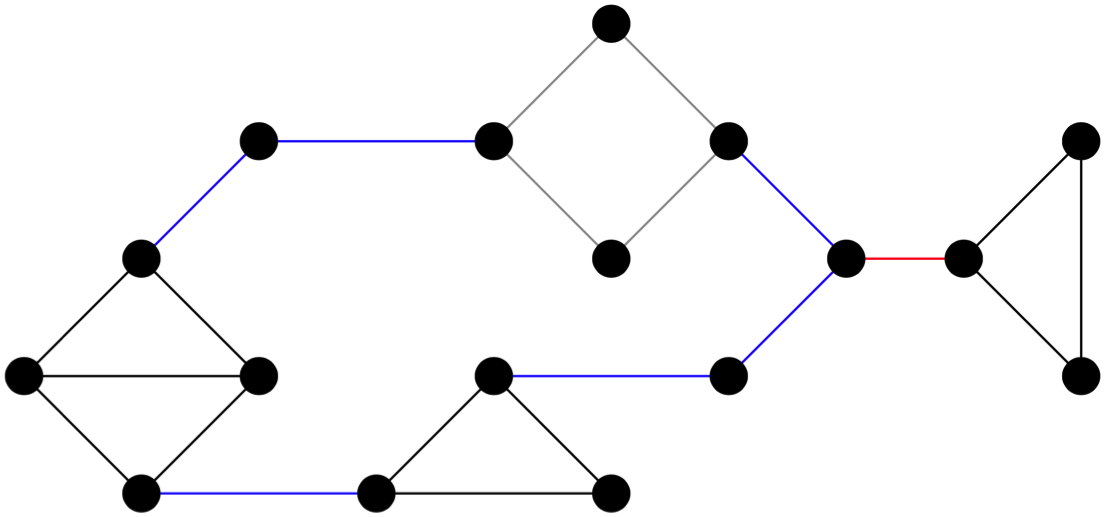
\includegraphics[width=0.85\textwidth]{Images/networkbridge.png}
\caption[Strong ties, weak ties, and network bridges]{Network highlighting a network bridge in red, structurally weak ties in blue, medium strength ties in grey, and strong ties in black.}
\label{fig:networkbridge}
\end{figure}

Although Burts' theory focussed on an individual as opposed to a firm or other non-personal entity, there are perfect examples of institutions and other non-personal entities which act as network bridges or middlemen. These include financial institutions and firms such as Google and eBay. Indeed, eBay acts as a network bridge, or a middleman, between groups of buyers and sellers. In doing so, the agent reduces search costs (or more generally, transaction costs) between the two otherwise unconnected groups of individuals and receives network effects from the increasing use of eBay from both buyers and sellers. Because of the structural location of a Burtian entrepreneur, they could simply be seen as a market-maker, and thus a direct middleman of relational interaction and trade.

The network bridge theory of the entrepreneur does not explicitly express the creation of new products, processes or professions in society. It is simply a story of arbitrage and resource allocation through the entrepreneurial function. However, the dissemination of information and the exchange of ideas are typically required for the development of new technologies which can be easily integrated into this perspective. Indeed, it is notable that Burt's postulation did not come to an end with providing the positional theory of the entrepreneur. He extended the structural hole theory in a more philosophical and less formal way; primarily focusing on the generation of new, innovative ideas \citep{Burt2004}.

% Emiliya: Typo (diverse and even contradictory information and interpretations provides them an advantageous opportunity -->  diverse and even contradictory information and interpretations that provide them an advantageous opportunity)

The core of his argument was that agents with bridge relations are critical to learning, creativity, and dissemination. Agents whose set of links span structural holes have unique access to diverse and even contradictory information and interpretations that provide them an advantageous opportunity in forming and exploiting good ideas. Undoubtedly, ideas come from a variety of sources; but, at some point, idea generation involves moving specific knowledge and information from one group to another, bringing agents together, or combining knowledge across groups. This process of the entrepreneur alludes not just to the brokerage of information, but rather to the arbitrage, recombination and practical application of specific knowledge and information; the result of which may lead to the formation of a new firm. Burt furthers his proposition by suggesting that agents who have network bridges across multiple structural holes and multiple divisions of labour are more likely to have their ideas evaluated \citep{Burt2005}. Indeed, social networks are effective tools for filtering and criticising good ideas---with more people evaluating an idea there is a greater chance for a good idea to emerge. Moreover, value accumulates as an idea moves through the social structure and divisions of labour; each transmission from one group to another has the potential to add value. This idea dissemination allows for the creation of a tight feedback loop, which is needed for successful invention.

Therefore, people whose links span multiple network groups have a competitive advantage in the creation of good ideas. An idea in one group may be extremely valuable in another. An idea is only really valuable to agents and entities when the audience credit it with being. This is more likely when ideas are diffused, discussed, and evaluated throughout society. Although Burt did not discuss it, this idea generation by spanning multiple networks could be the beginnings in which to investigate the disruptive Schumpeterian entrepreneur.

\section{Relational perspective of entrepreneurship}
\label{sec:RPEntrepreneurship}

The established theories are of two main strands. The first describes entrepreneurial actions that are shorn of institutional surroundings but respect the importance of positional opportunities. The second describes the relationship between institutions and entrepreneurship, which we discuss immediately below. Institutions are seen to provide the relative payoff structure that guide entrepreneurial actions and thus affect the allocation of entrepreneurial talent. Further, entrepreneurial activities can impact the context of institutions and the incentives that they provide to the economy as a whole. Such theories complement the relational perspective; specifically, the theories follow the directions of the schematic given in Figure~\ref{spacestructure}. 

An important, and often omitted, component is the acceptance that productive entrepreneurship stimulates an extension of the division of labour and facilitates increased specialisation---as discussed by \citet{Smith1776}. This leads to the development of new socio-economic roles, new exchange architectures, and new forms of interaction. This reengineering of the socio-economic space provides the basis for greater interactions and the development of new innovations. A feedback loop between the extension of the division of labour and entrepreneurial activity is implied. Entrepreneurship actively deepens the division of labour by both directly and indirectly providing more socio-economic roles through the alteration of the elements of the governance system. This is done through, for example, the provision of new products or processes or the reconstruction of exchange networks and the reorganisation of trade---much like the Schumpeterian perspective. By using the established theories of the entrepreneur we provide an integration of the notion of entrepreneurship to the relational perspective discussed. The focus in this section is on the interaction between entrepreneurs and the governance system, and how their activities generate new positions within the socio-economic space. We first elaborate on how institutions impact the incentives and actions of economic agents.

\subsection{Institutions and entrepreneurship} \label{entrepreneurshipInstitutions}

The governance system contains all established socio-economic roles within society and therefore defines the depth of the division of labour. Further, the structure of the accepted governance system and institutions provide relative payoffs to society and coordinate a socio-economic space of interacting agents to some steady state. The notion that institutions guide agents to some equilibrium is not a new phenomenon. It is well accepted in many schools of economic thought that institutions provide the payoff structure of society: that agents follow the payoffs provided by institutional frameworks, and that the rewards are generated by the actions correlate directly to institutional frameworks.

\subsubsection{Institutional impact of entrepreneurship}

% Emiliya: `Ill-defined institutions` need a better definition

Entrepreneurial activities are affected by the incentive structure provided by governance systems and institutional frameworks. One of the most influential discussions regarding the relationship between institutional environments and entrepreneurship derives from \citet{Baumol1990}. Baumol contests Schumpeter's perspective on the entrepreneur: that the entrepreneur is an individual who productively drives economic development and prosperity through waves of creative destruction. Baumol instead observes that the distinct form of entrepreneurship within a society is determined by the institutional structures of that society; and thus integrates institutional structures into the analysis of entrepreneurial action. Baumol's claim is that many historical institutional environments and arrangements have been more compatible with productivity-increasing technological innovations than others, however he notes that entrepreneurship has not always been of the productive variety. Institutions tend to determine both the level and type of entrepreneurship and Baumol identifies three types: productive, unproductive and destructive. Institutional pathologies may ensure that payoffs are skewed towards rewarding redistribution favouring sectional interests rather than in return for productive entrepreneurship. Dysfunctional institutions, those that they are ill-defined or provide poor incentives, may provide a basis for entrepreneurs to exploit\footnote{Within this context, `ill-defined institutions' refer to socially developed rules imposed on the actions of individuals and groups that are poorly enforced, contain unclear information, provide perverse incentives or intended consequences, or allow for rent-seeking activities.}. These institutional frameworks may provide incentives for entrepreneurs to rent-seek--lobbying for barriers to entry or exploiting employment loopholes--as opposed to expending resources into more productive and socially beneficial endeavours. Institutions may be operating with such malfunction that they are created only to be exploited by entrepreneurs that will ultimately damage the wider economic performance of the economy.

Others have extended Baumol's insights in more general terms. \citet{Murphy1991} is concerned with the allocation of talent within an economy and the impact that this has for economic growth. The authors are interested in how the most talented choose to seek returns and how incentives in a society promote rent-seeking or profit seeking. As such, they introduce factors that encourage rent seeking and productive entrepreneurship. Productive entrepreneurship, much like Baumol's discussion on the issue, requires large markets for goods, good communication and transportation infrastructures that facilitate trade, low barriers to entry and expansion, accessible capital markets and sources of finance, clear property rights, patent protection, and an ability to start firms that can make rents on talent. Again, talented individuals are, due to their embeddedness, assumed to abide by the institutional framework and respond appropriately to them. \citet{Acemoglu1995} extends the thesis posed by Baumol and the work of Murphy, Schleifer and Vishny by finding that the reward structures that determine the allocation of talent are endogenous. The endogeneity of this allocation of talent allows for the existence of path dependency such that initial differences in rewards and/or allocations will have long-run effects as allocations of one generation shape the rewards for the next. In concluding Acemoglu argues that there can exist situations in which two-way causality between the rewards structures of society and the allocation of talent. Indeed, these may occur in some historical examples.

\subsubsection{Interaction between institutions and entrepreneurship}

The schematic provided in Figure~\ref{spacestructure} claims that entrepreneurship works to affect the institutional environment of the economy, and thus works in the opposite direction of embeddedness. Institutional frameworks provide the payoff structures for individual agents; which ultimately provides a reinforced equilibrium for the society of agents. Institutions form an embeddedness that is unidirectional; abiding by pressures and payoffs from an existing set of institutions is the opposite of how entrepreneurship is perceived within our framework. As a consequence, we would contend that Baumol's perspective is not a perspective of the entrepreneur, and thus entrepreneurship, at all. We come to this contentious point due to two broad reasons. First, Baumol does not appropriately define what entrepreneurship is within his remodelled framework. The actual role of the entrepreneur is unclear. Of course, this is not necessarily a deficiency of Baumol's work as it is of notable debate in entrepreneurship literature as a whole. Second, Baumol perceives the entrepreneur as an agent that responds to the payoff structure defined by institutional pressures without actively altering the environment in which they operate. 

With regards the second point, Baumol's analysis indicates that institutions can determine the balance between productive, unproductive, and destructive actions undertaken by entrepreneurs. However, as noted by public choice theory and as was indicated by Acemoglu's work, feedback loops can exist whereby opportunistic individuals can actively alter the institutional environment they operate in to improve their own payoffs. This is indeed the essence of entrepreneurship illustrated in Figure~\ref{spacestructure}. Entrepreneurship acts in the opposite direction of embeddedness: entrepreneurs modify the institutional environment that they operate in; the outcome of which can lead to positive outcomes for themselves, and potentially for society as a whole. Whether the entrepreneurial agent alters the governance system in a productive or unproductive way will largely depend on the institutions already in existence within the economy.

This interaction between institutions and entrepreneurs is somewhat captured in the work of \citet{HenreksonSanandaji2011} who integrate James Buchanan's insights into Baumol's model of the entrepreneur. \citet{Buchanan1980} noted that entrepreneurs can affect institutions in multiple ways, by: 
\begin{itemize}
\item[(i)] Market innovations that alter institutions or the effect of institutions; 
\item[(ii)] Evasion of institutions; and 
\item[(iii)] Direct political entrepreneurship. 
\end{itemize}
Just as Baumol noted that the supply and allocation of entrepreneurial talent depends on the institutional framework of society and therefore the relative payoffs to profit seeking and rent-seeking activities, Henrekson and Sanandaji note that the allocation of entrepreneurship depends on the ability for agents to abide, evade, or alter institutional frameworks. Moreover, they acknowledge that the same individual can switch between different forms of behaviour.

This bidirectional relationship extends Baumol's perspective and leads to the notion of \emph{institutional and political entrepreneurship}. This is not a new notion as discussed by \citet{BoettkeCoyne2009}. Initially, \citet{Dahl1961} discussed individuals who recombine resources in an effort to bring about change in policies that effect the wider economy. Within Dahl's framework, political entrepreneurs are effectively Schumpeterian entrepreneurs acting within the political space. A distinction is made between so-called political entrepreneurs and market entrepreneurs, who, ``refer to traditional Schumpeterian entrepreneurs, distinct from political entrepreneurs'' \citet[p.~50]{HenreksonSanandaji2011}. The authors claim that not only is there a distinction between these types of entrepreneur, but that they are interdependent: political entrepreneurs must create the environment for market entrepreneurs. The economic system can thrive or collapse as an outcome of the actions provided by political entrepreneurship. \citet{Eisenstadt1980} and \citet{HwangPowell2005} discuss `institutional entrepreneurship' which involves entrepreneurship over the structure of government--i.e., decisions regarding the general institutions within which ordinary politics take place. Institutional entrepreneurship specifically involves changes to the fundamental constitution of the formal and informal rules of the game. \citet{DiMaggio1988} used the term institutional entrepreneurship in reference to those individuals who have the resources and ability to generate changes in institutions. Institutional entrepreneurs can be driven by a variety of factors including monetary gain, prestige or power. This discussion of the entrepreneur extends beyond the political sphere of the economy, and focuses on more ingrained institutional features, such as informal rules of the game, including beliefs, behavioural rules, religion, and scientific knowledge. Such institutional entrepreneurship may have a less obvious but more distinct and withstanding impact on society \citep{Abrutyn2013}.

In all there is some consensus regarding the phenomenon that entrepreneurs can impact the institutional architecture of an economy, whether that be from the political or the economic spheres of the economy. The impact of an entrepreneurs' actions on the institutional architecture can be either productive or unproductive depending on the payoffs of conducting these acts. A productive entrepreneurial impact provides an environment with greater market opportunities and subsequent wealth-generation within society, but requires the incentive structure for entrepreneurs to provide it. An unproductive or destructive entrepreneurial impact conversely provides an environment with more restricted economic activities and opportunities, where talent is allocated to rent-seeking as opposed to profit-seeking acts.

\subsection{The unique network positions of entrepreneurs}

In properly integrating the entrepreneur and entrepreneurship into the relational perspective we provide a discussion on the interaction between entrepreneurship, institutions, and the unique positional attributes that economic agents attain from the development of a new socio-economic role within the division of labour. Below we provide a deeper insight into entrepreneurship and the entrepreneurial function within the relational perspective by understanding the interdependencies between the advancement of socio-economic roles, the development of positional attributes, and the context of the institutions of the governance system.

\subsubsection{Entrepreneurship, new socio-economic roles, and unique positions}

Chapter~\ref{ch:relationalperspective} argued that the development of a social division of labour leads to the formation of social and economic positions. This is due to the network of relationships that form as a consequence of an individuals' specialisation and subsequent trade relationships. As such, individual economic agents will have a tendency to form similar socio-economic relationships given that they have similar socio-economic roles; there is positive assortativity in social and economic networks. We can therefore stipulate that, due to the the positional attributes of socio-economic roles and the novel nature of entrepreneurship, the formation of new socio-economic roles leads to the formation of a unique set of socio-economic relationships and thus a unique position within the socio-economic space. Indeed, by utilising Lemma~\ref{con:positionalattributes} and the discussion above we arrive at the conjecture below. 
\begin{conjecture}[Unique positions of entrepreneurs] \label{conjecture:UniquePositions}
Through a process of entrepreneurship an economic agent creates a new socio-economic role. This role carries unique positional attributes within the interaction infrastructure it exists.
\end{conjecture}
The uniqueness of an entrepreneurs positional attributes and the development of these unique positions fits well within the relational perspective and integrates some aforementioned theories of the entrepreneur; such as those from Smith, Schumpeter, and Burt.

Entrepreneurs therefore have access to higher levels of social capital with regards the formation of global and local bridges. Moreover, in extending Burt's insight we note that the entrepreneur adds value to this unique set of relations through entrepreneurial actions: specifically through the provision of an innovative output or production process that requires a hitherto unrelated set of specialisations and socio-economic roles; or through the potential rent-seeking and increased bargaining power that comes with brokering information and outputs. In some cases the entrepreneurial socio-economic role has some incentive to allow information to flow through the entrepreneur to other agents and specialisations; particularly with the formation of a novel output and the generation of ideas. In other cases, the entrepreneurial socio-economic role has some incentive to block the flow of information from one agent to the other; this may be the case where the exchange of knowledge does not directly benefit the entrepreneurial agent, or where the agent wishes to exploit some bargaining power to influence the institutions of society. The inherent institutional structure may affect the strategies of entrepreneurial agents; the governance structure of the space determines the actions of the socio-economic role.

\subsubsection{The interaction of institutions and network positions}

We have expressed two aspects of entrepreneurship thus far. First, the process of entrepreneurship can lead to the development of new socio-economic roles. As the division of labour deepens potential specialisation is extended and new positions are formed within the socio-economic space. Second, entrepreneurial agents form unique positions within the connected fabric of the socio-economic space and, due to their positional attributes, they can either be rent-seeking or wealth-generating with their actions. More generally, \emph{middlemen} can exploit their position within a network through the process of rent-seeking or can facilitate exchange between individuals and markets that were previously unconnected by providing a platform for interaction. Consequentially, entrepreneurial agents can act in a positive-sum, zero-sum, or negative-sum way \citep{Krakovsky2015}. Much depends on the context of the governance system and thus the relative payoffs to rent-seeking or profit-seeking actions. If institutions are ill-defined or if the rules of the game regarding the expropriation of rents from intermediating exchange are poorly enforced then the entrepreneurial agent has an incentive to act opportunistically. On the other hand, if institutions are imposed to effectively mitigate opportunistic behaviour, it incentivises these agents to be more productive with their positions and as a consequence add wealth to the network as a whole by facilitating exchange.

The example relating to the mortgage brokers of the Great Panic of 2007/2008 contends that the institutional environment needs to be established in order to reduce the unproductive and destructive acts of the enterprising agents; particularly those actions of middlemen. However, the relationship between entrepreneurship and institutions is bilateral; we specifically contend that agents with high levels of social capital and unique positional attributes can influence a change to the governance system due to their increased bargaining power from their position. The institutional environment can be lobbied and modified by individuals and groups with unique positions in the socio-economic space. As such, productive entrepreneurship and profit seeking can naturally lead to unproductive or destructive entrepreneurship through rent seeking and the altering of institutions. Due to their positional attributes entrepreneurs will also have the opportunity to accumulate wealth and rents, potentially gaining economic prominence within the socio-economic space and using this prominence to impact the elements of the governance system.

\begin{framed}
\paragraph{An example: Financial brokers during the Great Panic of 2007/2008.}
The exploitive potential of agents in unique positions are particularly sensitive to the governance structure of the socio-economic space. As a simple illustrative example, \citet{Crotty2009} discusses the architecture of the financial system that evolved during the run-up to the Great Panic of 2007/2008. Whilst noting a number of theoretical problems that underpinned the financial crisis, Crotty also notes the perverse incentives and exploitative power given to mortgage and financial brokers. Without correct and well-defined institutional regulation on their actions clients were granted mortgages without being correctly scrutinied. Moreover, due to the commission basis in which mortgage brokers are remunerated, they have incentives to exploit their asymmetric information and unique role and connectivity in the financial structure. The rules of the game informed by the institutions of a socio-economic space provide incentives for the brokering middlemen to be opportunistic and therefore exploit their unique position. The brokers are pursuing destructive actions; they effectively rent-seek at the expense of society.
\end{framed}

In all, the creation of social and economic capital through entrepreneurial acts, the development of the division of labour, and the attainment of unique positions in the socio-economic space increase the bargaining power for individuals or groups that possess these positions. By monopolising the flow of information and/or outputs throughout a networked space one can gain economic prominence and affect the formal rules of the game. Unique positional attributes in a network of relationships through the extension of the division of labour are important for understanding the relationship between the three aspects of entrepreneurship, institutions, and networks.

\subsection{The fused nature of entrepreneurship}

The triple of network positions, entrepreneurship, and institutions are fundamental in the analysis of economic development through the extension of the division of labour. The notion of entrepreneurship under the relational perspective indicates that it is often difficult to partition these components of the triple: entrepreneurs create new socio-economic roles which provide them with new positional attributes and potentially high economic and social capital that can be leveraged to actively alter institutional elements of the governance system. Further still we can make the inference that, given the setup of the relational theory, elements of the established theories are fused. For example, disequilibriating product and process innovation has a fundamental impact on the elements of the governance system and also benefits from high levels of social capital through bridge formation specifically due to the acquisition of ideas and dissemination of innovations.

A purpose of this chapter is to illustrate how these concepts--network positions, entrepreneurship, and institutions--are interlinked. Their interlinked nature is captured by the rise of the House of Medici, which we turn to next. Further chapters provide measurements regarding the power of network positions and how individuals and coalitions of network agents attempt to gain network power, and how these individuals then influence changes to the institutional elements of the governance system.

\section{The relational entrepreneurship of the House of Medici} 
\label{sec:HouseofMedici}

Modern capitalism based on private property rights owes its origins to the Italian Renaissance. A notable achievement from this period was the conception of modern banking, which economic prominence relies on today. We provide a brief analysis of the roots of capitalist banking and the fruition of the incorporated economy and relate this analysis to the theories of relational entrepreneurship as discussed above. Of specific interest are the entrepreneurial efforts of the Medici family, particularly Giovanni di'Bicci de'Medici and his son Cosimo di'Giovanni de' Medici, both of whom are considered to be the fathers of modern banking due to their innovations in financial accounting and financial organisation as well as their political dominance throughout the Renaissance and the industrial revolution.

To begin this analytic narrative, and to trace the roots of modern capitalism and the European banking system, we must first provide a brief account explaining the consequences of the Black Death on Western Europe--with a particular concentration on Florence Italy. We do this to provide a setting for explaining the current state of the socio-economic space itself; the institutional make-up and environment for entrepreneurial activity. In particular we elaborate on the subsequent power-struggles which persisted throughout Northern Italy during the late 14th Century, the political and economic network disjunctures which consequentially emerged and the fracturing control of the Catholic Church on the financial sector. All of these shocks to the socio-economic space of 14th century Florence provided the opportunities for the Medici banking house to reign supreme.

The plague was relatively egalitarian in its impact. As such, the plague affected the lower classes of society including the lowest ranking members of both the government and Church who were pivotal for the evangelism of Christ and the enforcement of formal societal rules. Moreover, due to the plague, cities such as Florence became inhabited and ruled by a relatively consolidated oligarchy of elitist families whose power became unconstrained by workers guilds; some of which had dissolved completely in response to the effects of the Black Death. Indeed, it turned that despite its egalitarian impact, some of the best-off in society were able to shelter themselves from the exogenous shock and thus strengthen their power at the detriment of the rest of society.

The population of Florence grew quite quickly a generation later as the devastating effects of the Black Death subsided. However, the re-inhabitance of Florence led to a neighbourhood split in terms of both social class and political power. A large and evident wealth gap emerged in Florence, which was exacerbated by geographical proximity and a lack of institutions to facilitate the poor and stop the exploitation by the aristocracy. Indeed, the ruling oligarchy geographically separated themselves from the rest of society. This striking division was fuelled by inherited networks, class homophily, the confounding effects of the Black Death, and was also a sign of a societal tipping-point; a game theoretic equilibrium which reinforces segregation within society, also known as a separating equilibrium. However, such an equilibrium, although accepted in game theory was historically unsustainable in Florence due to the consequential perverse effects on fairness and the distribution of economic opportunities which were typically skewed to those already in power. Indeed, any government policy would inevitably be favourable to the oligarchic aristocracy rather than those lower classes in society. It was a socially undesirable equilibrium and thus proved to be unsustainable due to collective counteraction. This became known as the Ciompi Revolt.

\subsection{The re-organisation of the Florentine society}

The unfair socio-economic environment after the Black Death led to the Ciompi Revolt in Florence 1378. This was a revolution of the lower classes--where groups of wool carders, vegetable sellers and crockery vendors, known as the Ciompi, lobbied to demand a voice in the Florentine community's order due to their non-representation by a guild. The Ciompi Revolt had a lasting effect on the social, political and economic networks in Florence. In short, the revolution brought with it a gradual and lasting deterioration of the social stratification through a restructuring of marriage and economic networks, a partial liberation of the poor, and a favourable lean towards a truly democratic political system. Importantly, the Revolt split the incumbent oligarchic aristocracy in two: those who sympathised with and fought alongside the Ciompi, and those who didn't.

\subsubsection{The beginnings of the House of Medici}

The Ciompi Revolt in Florence is a fitting place in which to introduce the role of the Medici family. The roots of the Medici Bank stretch back to the Ciompi Revolt. Salvestro de'Medici (1331--1388), a cousin of Giovanni, was of extreme importance for initially paving the way for the ``House of Medici.'' His appointment as the \emph{Gonfaloniere of Justice} in July 1378 as a consequence of the Ciompi Revolt allowed him to begin promoting a reputable and respected name for the Medici. As the Gonfaloniere of Justice Salvestro was given a notable degree of power and subsequent access to the social network of the ruling aristocracy. During the time of his rule the money-lending bank of Vieri di Cambio de' Medici, the first cousin of Salvestro, was in its maturation stages of growth and was accepted into the well-established \emph{Arte del Cambio} guild in Florence specifically due to the influence of Salvestro. Due to the consequentially increased reputation of the Medici name, Vieri was continually approached to provide financial services to the municipal government of Florence and the Curia of the Catholic Church located in what is now considered Vatican City in Rome. Due to the trusting functional relationship that was established, the financial trade continued even after Salvestro ceased to serve as the Gonfaloniere of Justice.

Giovanni di'Bicci de' Medici (1360--1429) came from a separate family line than both Salvestro and Vieri. Although once being celebrated in Florence, Giovanni's side of the family experienced a colossal fall from grace; being associated more with low-life criminal activity. Giovanni, however, reaped fortune from misfortune: the death of his father from the Black Death and his subsequent orphaned state led to a de facto adoption by Vieri, who provided Giovanni with a job in his moderately successful bank. Thus, from fortuitous opportunities and lucky networking came the beginnings of the Medici bank.

A few years after the Revolt, in 1382, the Ciompi and artisan alliance was successfully overthrown by the partisan aristocracy. The counter-revolution conducted by the previous ruling oligarchs led to a further split between those of the aristocracy who sympathised with the Ciompi and those who did not. Those who strictly opposed the Ciompi eventually reigned over Florence for the remainder of the 14th century despite further intra-elite conflicts between families. The intra-elite factional struggles of the 14th century were so intense that each neighbourhood became geographically polarised into competing patrician neighbourhoods. In response to the Ciompi escalation the ruling oligarchs pulverised the losing Ciompi sympathising patrician side into structural isolates--detached houses with little or no social and economic connections between them. The searing revolt of the Ciompi placed a strain on neighbourhood solidarities. The elitist neighbourhood solidarity thus dissolved in the decades following the Ciompi Revolt.

When considering the social structure of the oligarchs after the Revolt, it can be seen that the aristocratic marriage networks shifted permanently during the period from 1385 to about 1420; from a quasi-feudal pattern of parallel, intra-neighbourhood marriage hierarchies, which had incorporated most patrician families, toward a citywide elitist pattern of intra-neighbourhood marriage cycles, which co-opted ``politically correct'' patrician families while structurally isolating patrician ``class-traitors'' who had collaborated with the Ciompi and artisan guild. The effect of this marriage transformation was to keep Ciompi-type challenges from ever arising again; to safeguard the now successful oligarchic aristocracy from another uprising. No longer were there fluid factions to play off one another. The progressive fracturing of all facets of society led to the creation of structural holes in the social network and the opportunity to span them in an entrepreneurial manner according to Burt. The Medici played a pivotal role in the restructuring of the marriage and economic networks that followed the counter-revolution. However, in order to explain their importance, we must first elaborate on the success of the Medici Bank under the control of Giovanni.

Giovanni's intelligence and prudence excelled him in Vieri di'Cambio's bank. His natural ability, desire and dedication to re-establish legitimacy behind the Medici name promoted him to become the manager of the bank's Rome branch. In this position he became one of the most trusted and highest ranked Papal money-lenders. However, the Medici bank remained second to the Alberti bank--the largest bank in Italy and the main recipients of the Catholic Church's fortune. In this regard, the Alberti's were the Medici's biggest competitors at the time.

Vieri stepped down from his bank in 1392, later dying in 1394. On his death the bank was immediately liquidated and his fortune was divided into three separate parts. All three amounts went to individuals who were within the same family as Vieri and went on to establish their own banks. However, only Giovanni's bank, which was initially set up in Rome, survived for a notable length of time. There are a few initial reasons why Giovanni's entrepreneurial effort was successful. The first is that the Alberti bank collapsed and the Alberti family expelled from Rome in 1393. Its collapse mainly derived from its hierarchical organisational structure which did not allow for flexibility and correct oversight of its money-lending practices. Specifically, the banks dealings in civil wars throughout Italy prior to the wars in Lombardi during the 15th century cemented its political disrepute and eventual collapse. Moreover, the Alberti family was seen as Ciompi sympathising during the Revolt and was thus punished after the successful counter-revolution. Secondly, Giovanni essentially took over Vieri's Rome branch under a different name giving him immediate access to a source of funds from the church's Curia. Finally, Giovanni could use other relations he had created and extended knowledge he has amassed when working in Vieri's bank to secure banking services across Italy. Interestingly, it is clear that the Medici banking network under Giovanni expanded where the needs of his social ties were greatest as opposed to his needs for economic value generation. Giovanni therefore took advantage of the information and opportunities that arose within his social and economic network.

\subsection{The rise of the House of Medici}

The success of the Medici Bank has been largely attributed to the entrepreneurial actions and organisational architecture established by Giovanni di'Bicci. Specifically, two main factors are prominent when considering the rise of the Bank. One factor can attribute to the accounting practices administered; particularly in the area of double-entry bookkeeping and also the commission placed on foreign exchange trades, which made financial services more profitable and set the stage for interest payments to be accepted by Christian lenders later. The other factor relates to the partnership system that was established, which provided the basis for a decentralised banking system spawning from Florence and then being adopted throughout Europe. Such a structure allowed for a vastly spanning relational network of credit ties under the Medici name. The decentralised nature of the Medici banks organisational architecture was particularly novel relative to the traditional banking across Europe during the Middle Ages. In Florence, many of the dominant banks that collapsed in response to the Black Death were unitary banks that operated solely in Florence. We assess both of these innovative factors in more depth below.

The first innovation to be discussed concerns the accounting technique developed, which ultimately evaded the usury doctrine stated in the Old Testament and imposed as an embedded rule by the Catholic Church. The imposition of the usury doctrine discredited interest-burdened money lending throughout Europe and ultimately meant that the construction of modern banking systems was largely impossible. The Medici Bank did not strictly perform money lending services; rather they were foreign exchange dealers who relied on Bills of Exchange in order to trade in multiple currencies. Their accounts highlight their reliance on these Bills of Exchange specifically because of their ability to impose implicit usury. The Church strictly prohibited the collection of interest on loans; the formal and informal rules of the game influenced the nature of banking and the architecture of banking organisations. However, traders could make money from transactions that included the exchange of multiple currencies. Therefore, instead of charging interest, the Medici Bank imposed a commission which was deducted from transferring one currency into another. If the money was in the hands of the trader for any substantial period of time then the charged commission would be larger. Subsequently, if depositors put their money into the bank they were given \emph{discrezione}--which referred to the return paid by the banker for this privilege and the risk that the depositor accepted. This was considered to be `credit', again discretely concealing the interest charged. This was one of the first times that deposits were ever created.

To earn discrezione the bank would claim the transfer of currencies without a trade actually occurring. This act of creative accounting was used as a mechanism to bypass the laws of usury. It proved to be in society's best interest. It was a progressive act, particularly favouring the oligarchic aristocracy and the Catholic Church who used the Medici to transfer money initially across Italy and then to the rest of Western Europe as Giovanni's banking network expanded. With the application and social acceptance of this entrepreneurial idea, Giovanni de' Medici evolved the institution of money lending into what would now be considered as the foundations of modern banking.

Henrekson \& Sanandaji suggest that entrepreneurs can evade and potentially alter society's institutions through their acts. We claim that the Medici Bank, particularly under Giovanni, altered the institutional configuration of Florence beginning with its embedded beliefs regarding the usury doctrine. The evasion substantially increased the payoffs of holding deposits and exchanging currency for bankers and allowed the Medici to amass supreme levels of wealth. From an evolutionary perspective, we may maintain that the evasion and ultimate alteration of the usury doctrine was a productive form of entrepreneurship. Moreover, discretzione was an embedded belief that became widely accepted throughout Florence and later adopted by other banking houses throughout Italy. Only through their social relations did the Medici's invention become socially recognised and embedded into the economic transactions of banking, therefore being accepted and imitated by the rest of society. We can see the acceptance of the Medici within Florence and the profession of money lending within society as a whole with the Renaissance paintings commission by banking houses, including the Medici. Indeed, Botticelli's \emph{Adoration of the Magi} and \emph{Portrait of a Man with a Medal of Cosimo the Elder} (shown in Figure~\ref{botticelli}) show the Medici family in a well-regarded and powerful manner. With the Medici family, banking went from being relatively stigmatised to being next to divinity.

\begin{figure}[h!]
\centering

\includegraphics[width=\textwidth,height=0.75\textheight,keepaspectratio]{Images/botticelli.jpg}
\caption{Botticelli's \emph{Portrait of a Man with a Medal of Cosimo the Elder}}
\label{botticelli}
\end{figure}

The second innovation was the organisational structure of the Medici Bank. The Medici used a different organisational structure than was typically seen in Florence during this time. Traditionally we would see centralised and hierarchical banking houses--like the Alberti bank. Due to the banks initial roots in Rome it quickly established a branch-based system in both Rome and Florence. Subsequently, the bank designed an organisational structure that was more decentralised and governed by a set of harmonised lending rules within all of its branches. This decentralised network allowed for the diversification of loans and ultimately the reduction of risk, which lowered the cost of banking. Their organisation reflected that of a joint stock company whereby the parent company, located in Rome, controlled the subsidiary partnerships by owning more than 50\% of the capital of its branches. Other partners also owned substantial amounts of stock within the subsidiary banks meaning that their compensation was tied in with the banks performance.

Instead of a salary branch managers were junior partners who received a share in the profits plus an allowance for living expenses. The system provided incentives for increasing effort levels and lowering risk-shifting. Moreover, a promotion system and hierarchy was obvious in that a satisfactory manager had a high chance of becoming a partner and thereby greatly increasing his earnings. The Medici did not have the power to dismiss the junior partners, but rather had the power to condemn partners at any time. In effect, the Medici Bank had created an organisational architecture similar to that of a limited liability holding company. Under this structure decision-making was decentralised and the risk burdened on the Medici was diluted by being differentiated across the activities of other branches. Moreover, the structure gave the Medici themselves easy oversight, a clear locus of control and therefore the ability to create rule sets that had to be accepted by the other branches.

It could be argued that the Medici's organisational structure evolved to adapt to transaction costs that were prevalent within the firm. Decision rights were decentralised throughout the organisation to make use of local information but, as a consequence, partners could be opportunistic with their resources and abilities. In particular, partners could damage the Medici's reputation and profitability through risk-shifting or through privately capturing the gains from lending activities. Partners within the organisation require monitoring and evaluation from central authorities; however monitoring and the transfer of information from Rome to Florence would be costly. The costs of monitoring partners were reduced through the incentive alignment that comes with providing partners from different branches stock in their branch. Decision management and control responsibilities become attached to the residual claimants of the firm.

\subsubsection{Social structure of the political and economic aristocracy}

The theoretical perception of the entrepreneur developed above highlights the importance of the positional attributes of economic agents for the exploitation of power and influencing change. Although the process and organisational innovations were pioneered by Giovanni, the positional power of the Medici within the Florentine aristocracy can be attributed mainly to Cosimo as a political networker. After laying the foundations, Giovanni stepped down from the bank due to illness and ownership transferred to Cosimo, Giovanni's son, who led the Medici family to political dominance. Cosimo consolidated political and economic power in an entrepreneurial manner by leveraging a central position in the networks of aristocratic family inter-marriages, economic relationships and political patronage. 

Cosimo's success was not specifically due to his superior business leadership, but rather to his superior networking ability and patronage of the arts which became of increasing importance as the Renaissance began to flourish. He was therefore multiply embedded in various aspects of the socio-economic space, playing a role in complex and overlapping Florentine marriage, economic, and political patronage networks. He was riding hard on vast macro-political and macroeconomic forces far beyond his control. Yet he founded a political dynasty that dominated Florence for over three centuries. He consolidated a Europe-wide banking network that helped induce both international trade and state making elsewhere. And he oversaw and sponsored the Florentine intellectual and artistic effervescence that we now call the `Renaissance'. Such sprawling success of a single individual is largely due to two factors: the economic success of the Medici Bank and Cosimo's positional power within the socio-economic networks present in Florence at the time.

We defined multivocality as corresponding to an agent who specialises in a number of different roles and therefore may directly operate in a number of different aspects of a socio-economic space. We use this definition of multivocality with an application to Cosimo de'Medici to explain the prominence of his position in the socio-economic space. To do this we must first note that the Medici benefited from the restructuring of the marriage networks which occurred over the decades following the Ciompi Revolt and subsequent counter-revolution. Marriage networks were strategically restructured in order to segregate those who sympathised with the Ciompi and those who did not: intra-elite marriages were conceived partially in political alliance terms and were used to strengthen the aristocracy's position such that further revolutions by coalitions of workers could not emerge again. The aristocratic families that did not sympathise with the Ciompi tended to marry with other non-sympathisers. This resulted in a tight-knit marriage network of socio-economic equals within their oligarchic neighbourhoods. Conversely, sympathisers called the ``New Men'', did not tend to marry into other sympathising families--each family remained relatively isolated.

\begin{figure}[h!]
\centering
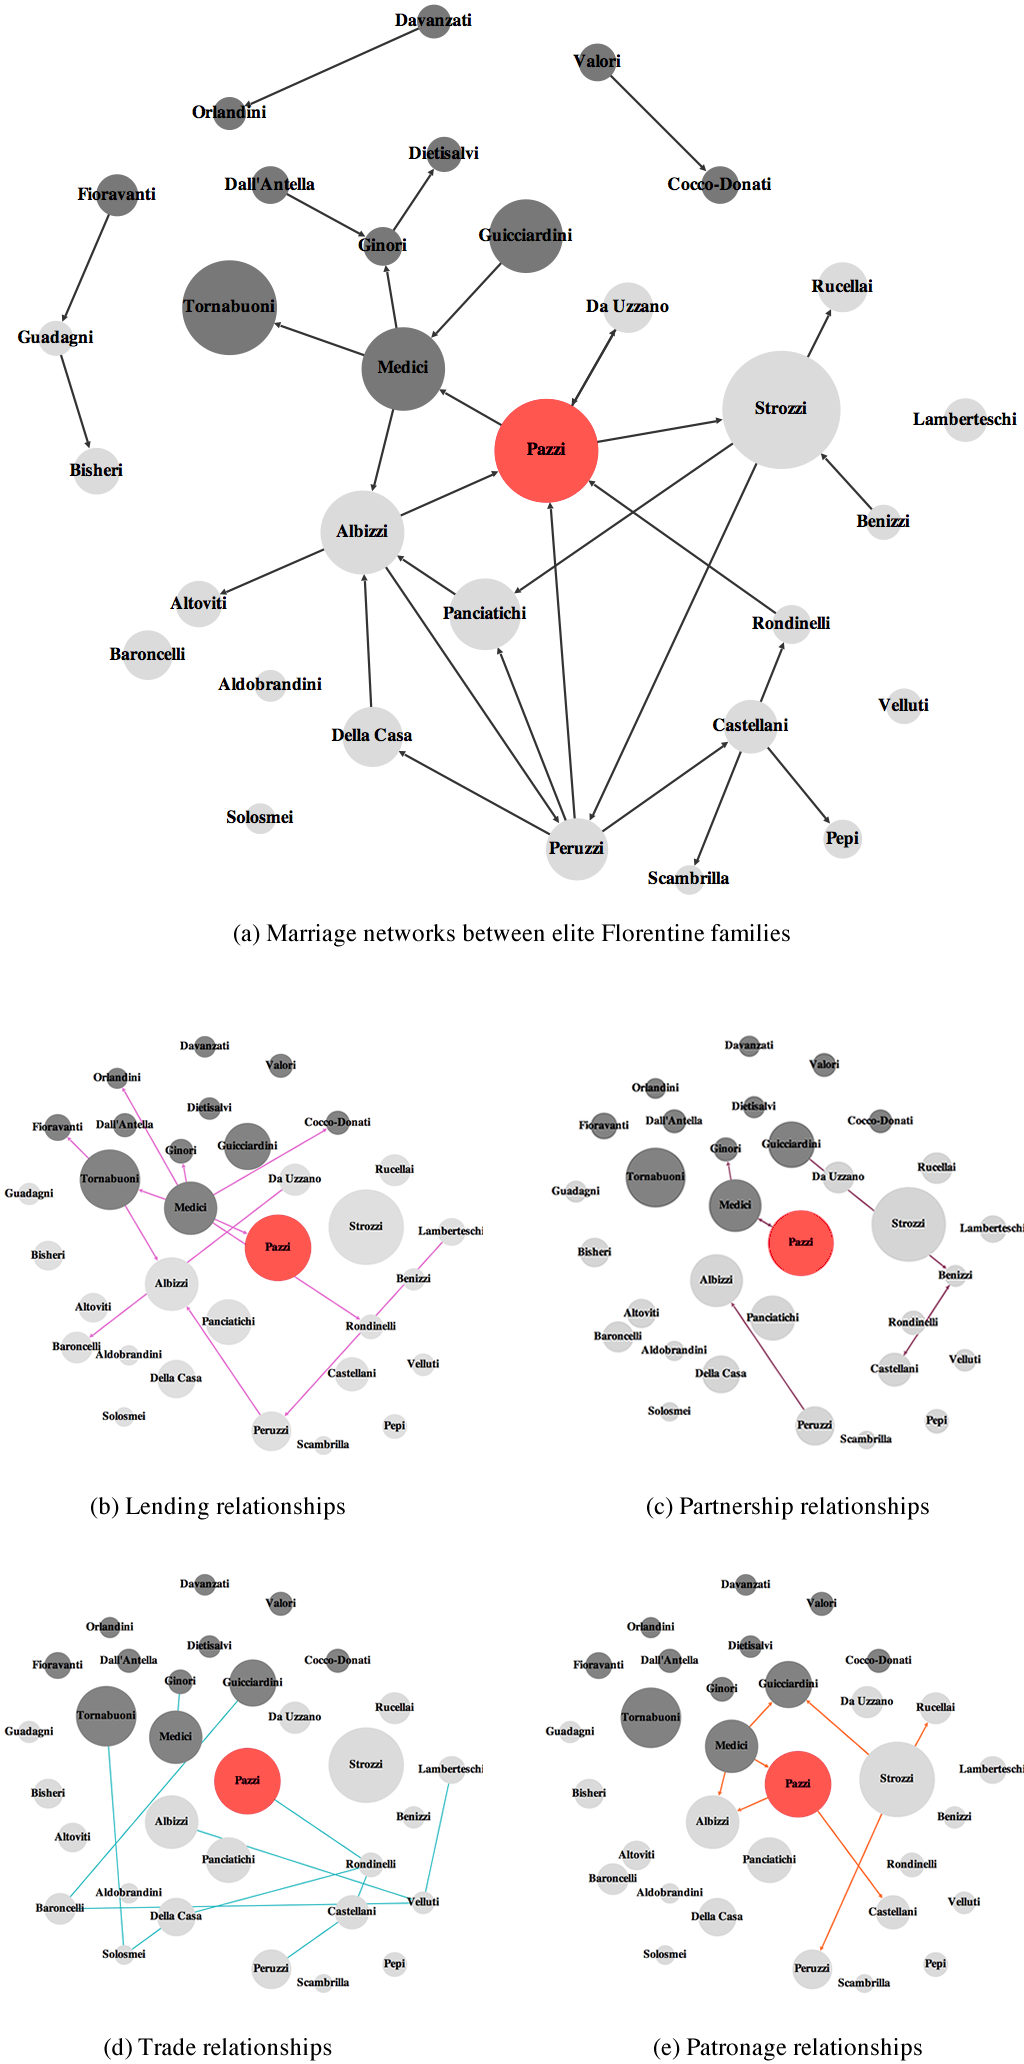
\includegraphics[width=\textwidth,height=0.9\textheight,keepaspectratio]{Images/allnetworks.png}
\caption[Social and economic relationships between aristocratic Florentine families]{Networks highlighting social and economic relationships that existed between aristocratic Florentine families circa 1429. Data gathered from \citet{Kent1978}, \citet{Padgett1993} and \citet{Padgett1994}.}
\label{florentinenets}
\end{figure}

The Medici's neutral stance during the period immediately after the Ciompi Revolt--as well as their aforementioned business and social success due to Giovanni's innovations--made them attractive to both sides of the oligarchic aristocracy. Over time the Medici, both strategically and fortuitously married into both sides and the resulting position in the social network allowed the Medici family to build and control an early forerunner to a political party, while the other families of the time suffered from internal power-struggles. It must be reminded to the reader that all of the aristocratic marriages recorded here were strategically arranged by patriarchs or their equivalents in the two families. As \citet[p.~1259]{Padgett1993} describe it, ``[the] Medician political control was produced by network disjunctures within the elite, which the Medici alone spanned''. Such a claim is evident with the aid of the set of graphs in Figure \ref{florentinenets}. This Figure provides five networks on the same set of families. Each network concentrates on a certain type of relationship. Specifically, network (a) shows marriage relationships that were strategically formed between families, network (b) shows the lending relationships between the families, network (c) shows partnership relationships, network (d) shows bilateral trade relationships between these families, and network (e) shows patronage relationships. The marriage network, the loan network, and the patronage network all indicate that the Medici filled a structural hole between the two opposing sides in both a social and an economic sense. Cosimo created a new and unique socio-economic role through his network position; a de facto ``president'' of Florence who, although never occupied office, had complete control of the political and therefore the institutional and economic environment of Florence and Northern Italy.

There are two interesting points to note with regard to the above marriage network. The first point highlights the importance of the composition of both marriage and economic linkages within the families in Florence. Each family's respective actions depended not only on independent rationalised decision-making, but also on how they are interlinked. It can be seen that power and influence reverberated through the marriage linkages meaning that the very composition of the marriage network within these families matters. When considering the ``New Man'' revolution of 1429, when the ostracised traitors rebelled against the oligarchic aristocracy, it became apparent that the dense structural interconnectivity of the oligarchic elite rendered them highly disorganised as control was decentralised through the marriage network. Power struggles emerged with so many intertwined socio-economic equals. The collective-action problem remained as they failed to realise a focal point in the form of a leader who could strategise and initiate action. The composition of their network thus affected their cohesiveness in times of crisis; each family schemed with other families to which they were tied as to the best course of action. Opposing stratagems arose between the different inter-linked families, ultimately generating tensions between the ruling elites as opposed to the necessary robust action. In effect, they became bound by their own network. Social ties can provide constraints as well as opportunities when individuals pursue their own self-interest without any clear governing rule-sets or leaders.

Whilst the oligarchs hesitated, the Medici was able to solve their collective action problem and mobilise their party. This was largely because of the composition of the marriage network underlying the party which centralised around the Medici. Indeed, the Medici were married into three other families directly, the Tornabuoni, the Ginori and the Guicciardini; this was combined with the fact that the other member families were not heavily interlinked through marriage as was witnessed with the oligarchic partisans. This provided a focal point which allowed for collective action. Such a situation provides an empirical basis in which to appreciate the power-dependence literature \footnote{For a seminal discussion on this literature see \citet{Emerson1962}.}. It is easy to appreciate how the dependence on a powerful and respectable family would be needed for collective action.

The second point highlights the entrepreneurial characteristic which brought the Medici family and Cosimo to power. The characteristic specifically refers to the Medici's centralised position within the social network of the ruling aristocracy. As seen above, the Medici family developed a star network which spanned both the oligarchic partisans and the Ciompi sympathisers. Such a position meant that followers of the Medici could only interact with the rest of the followers through mediation of the Medici. Moreover, if they wished to discuss issues with the oligarchic rulers, all information had to pass through the Medici and vice versa. From their strategic position in the social network they were able to remain in power as brokers of important information. To signify the powerful role of the Medici Pope Pius II claimed: ``Political questions are settled in his [Cosimo's] house. The man he chooses holds office... He it is who decides peace and war and controls the laws... He is King in everything but name'' \citep{Hibbert1980}.

\section{Concluding points and future discussions on socially structured economies}
\label{sec:ConcludingPoints}

Henrekson \& Sanandaji highlight the interaction between political and market entrepreneurship. In doing so they explain how the economic and political spheres of the socio-economic space can interact with each other and facilitate development. Particular attention is paid to how institutional entrepreneurs can affect the rules of the game and therefore the relative payoffs to, and allocation of, entrepreneurial activity within the economy. This interdependent development is illustrated by the authors specifically with the example of Silvio Berlusconi, who used his economic power from market activities to fuel his political dominance in Italy. His media empire throughout Italy provided him a platform to advertise himself, distribute his policies and influence the beliefs of the voting citizens of Italy. The outcome of Berlusconi's efforts can be labelled as unproductive and potentially destructive to society's welfare: indeed, there is evidence to show that throughout his business career he has used his political ties to seek and capture rents. Through market innovation the actions of entrepreneurs can influence a change to the institutional setting of the economy: this can be a consequence of direct or indirect effects. The interaction between market and political spheres of the socio-economic space is also notable with respect to the success of the Medici family. Furthermore, although not discussed by Henrekson \& Sanandaji, we suggest that the positional attributes of individual agents impact their power to influence the institutional environment of the socio-economic space. This is particularly apparent with the aforementioned network regarding the Florentine elite and the theory of relational entrepreneurship: Cosimo and the House of Medici influenced institutional change and the actions of elite Florentine factions primarily due to their positional attributes, which were formed as a consequence of their market entrepreneurship.

The above perspective of relational entrepreneurship extended the insights of Henrekson \& Sanandaji, noting that the position of an individual agent within a networked socio-economic space can inform their ability to broker information and exchange, and thus potentially gain a powerful position within a network. As such, entrepreneurial agents can form and exploit unique positions within a network, which can subsequently have an institutional impact. The unique position attained by entrepreneurial agents, as discussed throughout the monograph, can emerge as a consequence of the development of new socio-economic roles. As such, the relational perspective provides a way to investigate the interaction between these three important elements: institutions, socio-economic networks, and entrepreneurship. The interacting elements of institutions, socio-economic networks, and entrepreneurship can be easily applied to the case of the Medici as discussed thus far.

In fact, this is a purpose of the next Chapter of the monograph. Inspired by the stipulation made in Conjecture~\ref{conjecture:UniquePositions} we investigate further the notion of a entrepreneur by equating it to that of a \emph{middleman}: an agent that holds a unique position within a network. The uniqueness of the entrepreneurs position is determined by the paths within which it operates. We provide measurements of an entrepreneurs power within the network of relations and show that multiple agents can form middleman positions through entrepreneurial actions.
